\section{EXPERIMENTS}

\begin{figure*}[!ht]
\makebox[\textwidth][c]{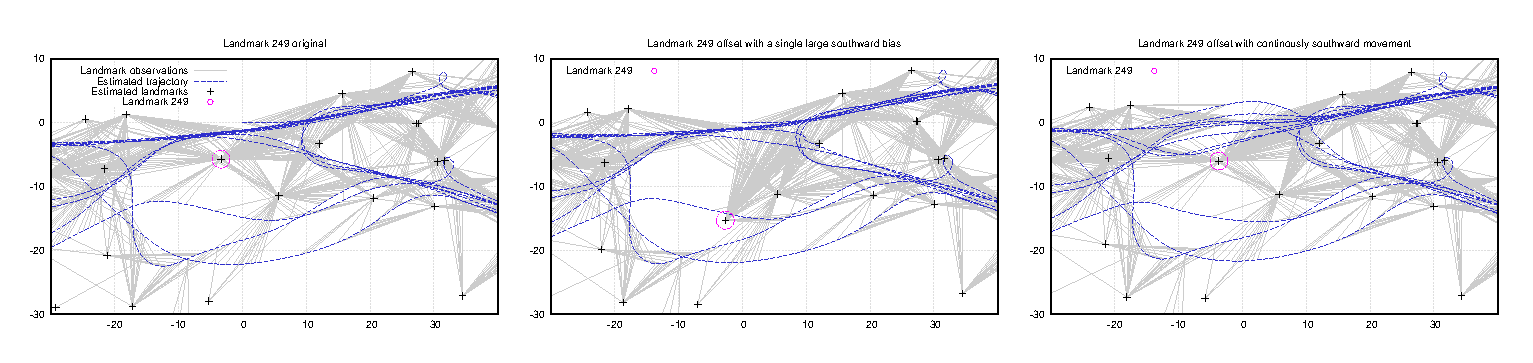
\includegraphics[width=\textwidth]{fig/baseline-mm}}
\caption{The optimal estimates of the trajectory and landmark positions
obtained by Max-Mixture graph SLAM.  Left: low convergence uncertainty
(measured by objective value). Middle: high convergence uncertainty because of
rejection of outlier observations of landmark 249.  Right: low convergence
uncertainty, no outlier detected by Max-Mixture.}
\label{fig:baseline}
\end{figure*}

We implemented our method as discussed previously and compared the result with
various alternative approaches. Our implementation is based on the graph
optimization framework g2o~\cite{g2o}, and we programmed a plug-in type library
in C++ to represent our modified objective function while reusing the Gauss-Newton
optimization functionality. The type library exposes properties of the edges including
the error metric, reweighted information matrix, and robust Mahalanobis distance function.

\subsection{Datasets}

The first dataset is the commonly compared landmark-based dataset Victoria Park released with iSAM~\cite{isam}. We apply different types of simulated corruption to the dataset to
generate multiple synthesized datasets to evaluate the effect on different
approaches.  For the purpose of evaluating performance against moving
landmarks, several other commonly used datasets are not suitable because they
are pose-only graphs without landmarks. The Victoria Park dataset of 2-D
odometry and landmark observations contains 6969 robot poses, 6968 odometry
measurements, 151 landmarks, and 3640 landmark measurements obtained.

% resolved \cj{in-door $\rightarrow$ indoor}
The second dataset is based on a set of real world data collected in crowded
environment at the Alcazar of Seville with a lot of tourists~\cite{iros14-frog}.
The original datasets provide wheel odometry, stereo images, and laser scans.
In the indoor GPS denied environment, the provided ground truth map and
trajectory are built using a non-linear batch optimization-based SLAM method
with an approximate accuracy of 20 cm. We extract potentially moving landmarks
from a indoor subset of this dataset through a standard pipeline of feature
detection and extraction, feature correspondence, and stereo estimation of
keypoint depth implemented with OpenCV~\cite{opencv} and ROS~\cite{ros}.%resolved\cj{do you have a citation for this pipeline? or some implementation detail, like a C++ implementation using OpenCV libararies? xlz: citations add, but how to cite OpenCV?}  
Due to lack of visual detection of loop closure, we also add
in a loop closure obtained from laser scans instead of image data at the
start-end point. This dataset tests the typical scenario of visual SLAM with
wheel odometry. The extracted dataset consists of 4892 robot poses, 5808
measurements, and 13454 measurements.

\subsection{Prior Methods with Moving Landmarks}

In the first test, we evaluate the performance of the state-of-the-art robust
SLAM method, a implementation of Max-Mixture~\cite{mm}, given dynamic landmark measurements.
Max-Mixture is a robust extension to classical graph SLAM using Gaussian
mixture in factor representation, that is, $ x_i = \sum_c \phi_c
\mathcal{N}(\mu_c, \Sigma_c)$ for component $c$ and weight $\phi_c$, with
observations being components, also similarly for $z_i$. Max-Mixture uses a max
function to approximate and efficiently evaluate the sum of Gaussians. It is
well-known for its capability of handling a large amount of incorrect loop
closures, but it is untested against moving landmarks, and this experiment can
be representative to other approaches in the robust SLAM literature. 

We apply different perturbations to all observations associated with a certain
landmark which has the most observations associated in the dataset, and study
the different effects of the perturbations on the optimal estimate of the
trajectory and the map of all landmarks obtained by Max-Mixture graph SLAM. The
Victoria Park dataset contains 2-D odometry and landmark observations. As shown
in Figure \ref{fig:baseline} the left plot is the control group without
perturbation, and is accurate to the ground truth. A single southward bias is
applied to all observations of the landmark in the middle plot, simulating
sensory outliers. A temporally increasing bias is applied to all observations
of the landmark in the right plot, simulating a southward moving landmark.

As the middle plot shows, Max-Mixture is still capable of handling noise of
large bias or spurious loop closures introduced by simulated sensory fault. It
correctly rejects outlier landmark observations and recovers the position of
the perturbed landmark. However, it completely fails to reject any unlikely
landmark observations and largely distorts the resulting trajectory when given
moving landmark measurements. An explanation for this is that each clique of
landmarks with coherent motion forms a plausible reference frame for related
observations. Inference based on each independent reference frame will reach
plausible estimate of robot trajectory and the map, however robust SLAM methods
which assume stationary landmarks will average over a sum of different
reference frames and lead to wrong conclusions.

\subsection{Comparison with Prior Methods}

To benchmark the robustness of the proposed approach and to show its
correctness and feasibility, we use the Victoria Park dataset that has been
used in a number of publications before. The dataset consists of pose graphs in
2D and contain several thousand poses and landmark constraints. We corrupted
the data by setting landmark ``249" (circled in red) in a constant northward
movement, where its eventual position is roughly 7 meters north of its original
location. We chose landmark ``249" due to the relatively large amount of
observations associated with this particular landmark in the dataset. We expect
the more observations there are on a landmark, the greater its movement would
corrupt the final optimization results and the more possible that existing
robust SLAM methods would fail.

\begin{figure}[ht]
\centering
\begin{minipage}[b]{0.48\textwidth}
  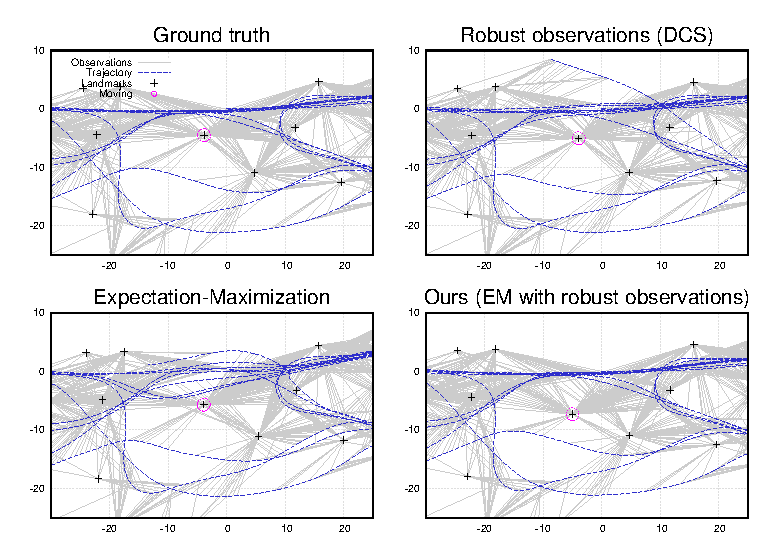
\includegraphics[width=\textwidth]{fig/small-movement}
  \caption{Dataset corrupted by the landmark with small movement}
  \label{fig:small-movement}
\end{minipage}
\quad
\begin{minipage}[b]{0.48\textwidth}
  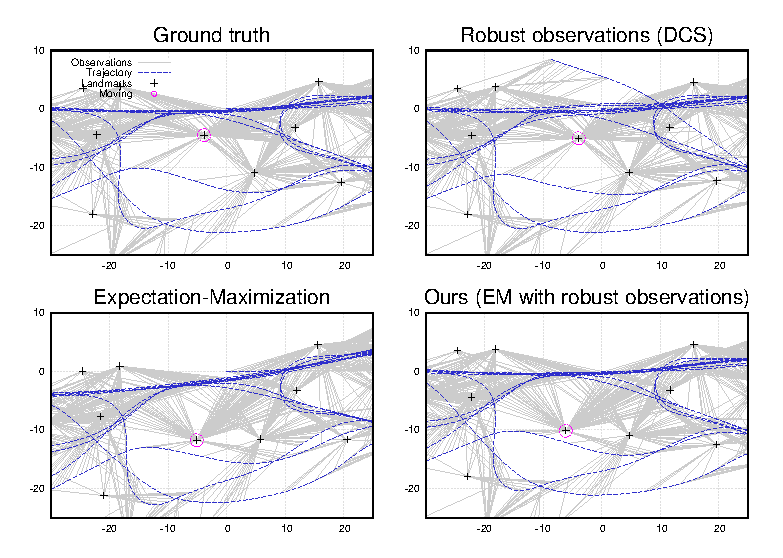
\includegraphics[width=\textwidth]{fig/large-movement}
  \caption{Dataset corrupted by the landmark with large movement}
  \label{fig:large-movement}
\end{minipage}
\end{figure}

We compare the results of Dynamic Covariance Scaling robust kernel as discussed in our
formulation, and also the SLAM with EM approach proposed in \cite{rogers2010slam}.  Figure \ref{fig:small-movement} shows the results for DCS, standard EM, and our
approach. As shown in the figure, robust observations alone are unable to
handle moving landmarks. Because observation-based robust methods do
not characterize the mobility of the landmark, its effect on associated
observations and assume independence between observations, which is not the case for moving landmarks. A moving landmark will cause associated observations to
be inconsistent in a plausible way such that a subgroup of the observations
might be able to converge to a local minimum but the rest of the observations
would distort the result elsewhere. 

Normal SLAM with EM was proposed in \cite{rogers2010slam} for datasets with
very large movement. Their formulation is similar with ours except it is
without the robust factor $v_k$.  As shown in Figure \ref{fig:small-movement},
the resulting trajectory is distorted. One explanation for this is from the
characteristics of the datasets.  In their paper, they investigated datasets
containing landmarks moved from one room to another room over a long period of
time.%, which is not the case in the Victoria Part dataset. 
%the dataset presented in figure \ref{fig:small-movement} 
Such long-duration mobility is not the case in the Victoria Part dataset, where the motion of the landmark is relatively small and continuous. In fact, %in figure \ref{fig:large-movement} 
the motion of the
corrupted landmark is doubled and normal EM is able to learn the mobility
correctly.

Our robust back-end however, is able to converge to a correct solution in a few
iterations. Our result is also verified by examining the learned parameters
$w_{j_k}$ and $v_k$ of all landmarks, which is close to zero for the actual
outlier landmarks, thus correctly deactivating associated corrupted
observations.  The improvement is explained by our utilization of the robust
kernel to make the EM algorithms reliably learn the mobility indicators of the
landmarks correctly identify the actual moving landmarks. Thus our approach is
able to obtain the best results in both situations.

In Figures \ref{fig:alcazar-robust} and \ref{fig:alcazar-movable-robust}, the
result also shows additionally comparison of different methods on the Alcazar of
Seville dataset. As can be seen, the trajectory estimation obtained with only
robust observations using DCS kernel is significantly distorted. Our method is
able to recover the trajectory approximately. The estimated trajectory does not
completely converge on the ground truth trajectory due to less than full
coverage of extracted landmarks and limited accuracy in depth estimation.

\begin{figure}[ht]
\centering
\begin{minipage}[b]{0.48\textwidth}
  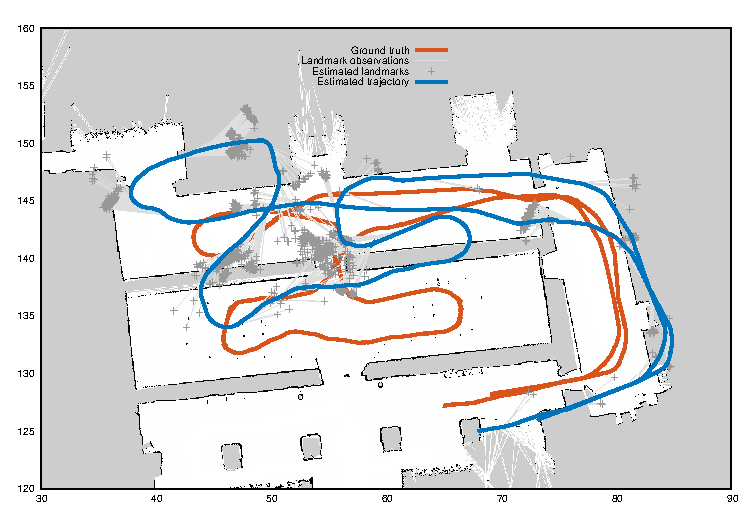
\includegraphics[width=\textwidth]{fig/alcazar-robust}
  \caption{Estimation with only robust observations (DCS) on the Alcazar of Seville dataset. Background is the ground truth map.}
  \label{fig:alcazar-robust}
\end{minipage}
\quad
\begin{minipage}[b]{0.48\textwidth}
  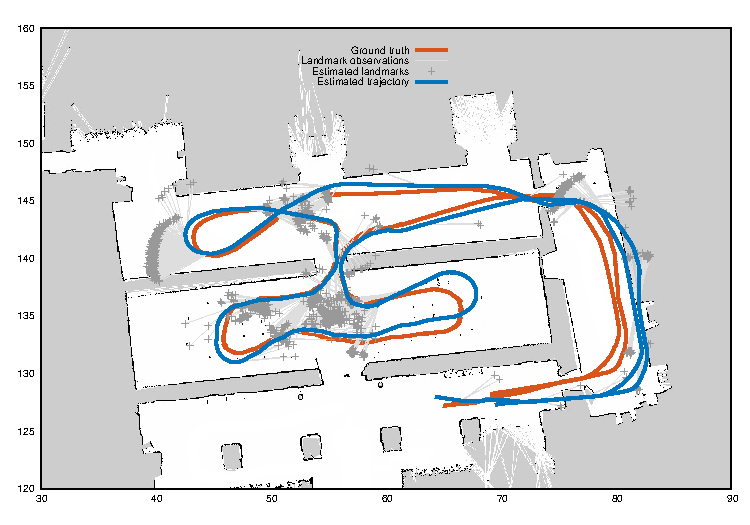
\includegraphics[width=\textwidth]{fig/alcazar-movable-robust}
  \caption{Estimation with our method on the Alcazar of Seville dataset.}
  \label{fig:alcazar-movable-robust}
\end{minipage}
\end{figure}

